% --------------------------------------------------------------------------------

\begin{exercise}[Exercise 3.24]

Figure \ref{fig:3.5} (below) gives the optimal value of the best state of the gridworld as $24.4$, to one decimal place.
Use your knowledge of the optimal policy and \eqref{eq:3.8} to express this value symbolically, and then to compute it to three decimal places.

\setcounter{section}{3}
\setcounter{figure}{4}

\begin{figure}[H]
    \centering
    \subfloat[Gridworld]
    {
        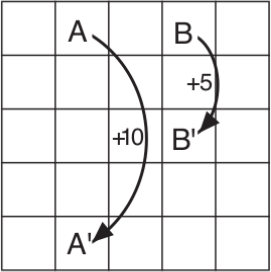
\includegraphics[width = 0.2 \textwidth]{1.21.1.png}
    }
    \hspace{1cm}
    \subfloat[$v_\ast$]
    {
        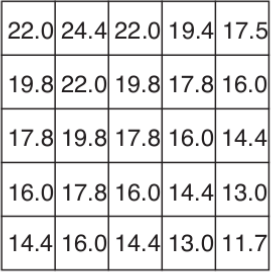
\includegraphics[width = 0.2 \textwidth]{1.21.2.png}
    }
    \hspace{1cm}
    \subfloat[$\pi_\ast$]
    {
        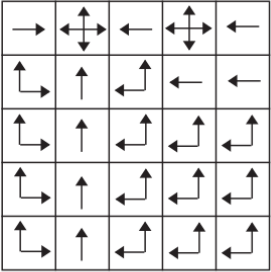
\includegraphics[width = 0.2 \textwidth]{1.21.3.png}
    }
    \hspace{0mm}
    \caption
    {
        Optimal solutions to the gridworld example.
    }
    \label{fig:3.5}
\end{figure}

\end{exercise}

% --------------------------------------------------------------------------------

\begin{solution}

Label the grid positions by $(x, y)$ where $x$ denotes the horizontal and $y$ the vertical position.
$(0, 0)$ should be located at the upper left.

The dynamics of $\pi_\ast$ are simple.
For each position $s$, after a certain number of time steps $t_s$, the player will always fall into the cycle

\begin{align*}
    A \mapsto A^\prime = (1, 0)
      \mapsto (1, 1)
      \mapsto (1, 2)
      \mapsto (1, 3)
      \mapsto (1, 4) = A.
\end{align*}

Note that $t_s$ is actually well defined because no matter what chain of actions (there may be multiple) is taken under $\pi_\ast$, the number of time steps it takes to move from $s$ to $A$ is always the same.
Before falling into that cycle, we collect some reward $r_s$.

\begin{align*}
    v_\ast(s)
    & =
    v_{\pi_\ast}(s) \\
    & =
    \E_{\pi_\ast}[G_t \mid S_t = s] \\
    & =
    \E_{\pi_\ast}
    \bbraces
    {
        \sum_{k=0}^\infty
            \gamma^k R_{t+k+1}
        \mid
        S_t = s
    } \\
    & =
    \sum_{k=0}^\infty
        \gamma^k \E_{\pi_\ast}[R_{t+k+1} \mid S_t = s] \\
    & =
    r_s
    +
    \sum_{k = t_s}^\infty
        \gamma^k \E_{\pi_\ast}[R_{t+k+1} \mid S_t = s] \\
    & =
    r_s
    +
    \sum_{k \in 5 \N + t_s}
        \gamma^k \cdot 10 \\
    & =
    r_s + 10 \sum_{k=0}^\infty \gamma^{5 k + t_s} \\
    & =
    r_s + \frac{10 \gamma^{t_s}}{1 - \gamma^5}
\end{align*}

\begin{verbatim}
    [[21.977 24.419 21.977 19.419 17.477]
     [19.78  21.977 19.78  17.802 16.022]
     [17.802 19.78  17.802 16.022 14.419]
     [16.022 17.802 16.022 14.419 12.977]
     [14.419 16.022 14.419 12.977 11.68 ]]
\end{verbatim}

\end{solution}

% --------------------------------------------------------------------------------
